\section{Мета, задачі і проблеми чисельного моделювання. Чисельне моделювання процесів гідродинаміки} 

\shortLectureDescription{Мета, задачі і проблеми чисельного моделювання. Чисельне моделювання процесів гідродинаміки. Основні закони та рівняння. Дивергентна і недивергентна форми запису системи рівнянь Нав'є-Стокса. Системи обезрозмірювання рівнянь. \emph{\cite{rouch1980, atp1990, sam1983}}}

\begin{figure}[H]
    \centering
    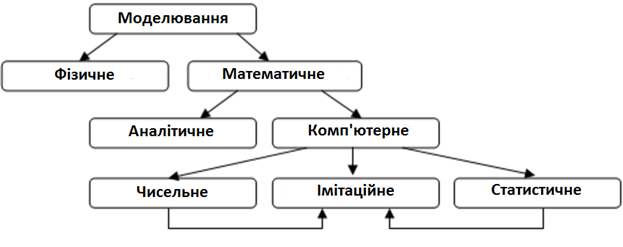
\includegraphics[width=.8\textwidth]{img/01/1.png}
    \caption{місце чисельного моделювання у моделюванні}
\end{figure}

Традиційно при \textbf{моделюванні} реальних фізичних процесів і проектуванні конкретних пристроїв одночасно використовувались \textbf{теоретичні} та \textbf{експериментальні} методи дослідження, за допомогою яких визначались основні характеристики процесів. З появою потужних ЕОМ з'явилась можливість використати третій підхід --- \textbf{обчислювальний експеримент}.

\subsubsection{Мета чисельного моделювання}

Обчислювальний підхід у моделюванні знайшов своє місце на межі між теоретичним і експериментальним, узявши на себе певну частину функцій як теоретичних, так і експериментальних методів. Іноді він дає змогу замінити високовартісні й довгострокові натурні експерименти чисельним моделюванням процесів на ЕОМ. Інколи такий підхід є єдиним можливим для визначення тих чи інших характеристик процесу. За допомогою чисельного моделювання можна прогнозувати поведінку, а варіюючи параметри --- встановлювати нові якості та закономірності протікання досліджуваного процесу, що здебільшого не під силу ані теоретичним, ані експериментальним методам.

\begin{example}
    Чисельне моделювання доцільно застосовувати у тих випадках, коли досліджувані процеси важко або навіть неможливо моделювати на макетах через їх велику швидкоплинність, надзвичайно малі геометричні розміри досліджуваного об'єкту, багатокомпонентність, надвисокі чи наднизькі тиски та температури середовища, а також в інших складних реальних ситуаціях.
\end{example}

При чисельному моделюванні реальних процесів множина \textbf{задач} як об'єкт математичного дослідження, вивчена недостатньо. Задача, в самому загальному розумінні, є ситуацією, яка визначає дії деякої розв'язуючої системи. 

\begin{definition}
    Розв'язуюча система є основним інструментом чисельного моделювання і класифікується як біологічна, технічна і комбінована система, до складу якої входять люди і автомати (машини). \medskip
    
    Ця система повинна мати технічні засоби розв'язування і теоретичні методи побудови розв'язку.
\end{definition}

\subsubsection{Класифікація задач чисельного моделювання} згідно із системою \guillemotleft{}людина --- автомат\guillemotright{} залежно від можливої ситуації така: 
\begin{enumerate}
    \item існує один або кілька алгоритмів розв'язування задачі, оформлених у вигляді програми, яка може бути реалізована на ЕОМ; 
    \item не існує програми для ЕОМ, але людина знає, як її побудувати; 
    \item не існує програми і невідомий метод розв'язування задачі. 
\end{enumerate}

У першому випадку задача зводиться або до вибору з множини алгоритмів найбільш придатного, або використання єдиного придатного алгоритму. У другому додається процес програмування відомого алгоритму (клас програмування). У третьому виникає задача розробки алгоритму і програми (клас задач синтезу алгоритмів).

\begin{definition}
    Якщо, починаючи розв'язувати задачу, людина не знає шляхів розв'язування даного класу задач, то таку задачу називають \textit{проблемною}.
\end{definition}

Розв'язування проблемних задач передбачає використання людиною додаткових евристичних засобів, відмінних від алгоритмів і алгоритмічних вказівок.

\begin{definition}
    Задачу назвемо \textit{добре визначеною}, якщо для неї існує алгоритм перевірки, який можна застосувати до запропонованого розв'язку.
\end{definition}

\begin{definition}
    Якщо інформації, що міститься в постановці задачі й самій розв'язуючій системі, достатньо для отримання розв'язку, то така задача є \textit{безпошуковою}.
\end{definition}

У пошукових задачах система повинна дістати додаткову інформацію із зовнішнього середовища. Вхідні дані задач поділяються на компоненти, які в умові описані досить повно (те, що дано в задачі), і компоненти, перелічені в умові задачі, але їх повний опис можна дістати лише після розв'язування задачі (те, що треба знайти). \medskip

Відповідно до процесу розв'язування задачі поділяються на такі типи:
\begin{enumerate}
    \item задачі \textit{виконання} (задано вхідні об'єкти, процедури; потрібно знайти продукти процесу);
    \item задачі \textit{відновлення} (задано продукти процесу, процедури; потрібно знайти вхідні об'єкти);
    \item задачі \textit{перетворення} (задано вхідні об'єкти, продукти процесу; потрібно знайти процедури);
    \item задачі \textit{конструювання} (відомо продукти із заданими властивостями; потрібно знайти відповідні вхідні дані та процедури).
\end{enumerate}
 
\begin{remark}
    Типовою дією, яку виконує розв'язуюча система, є виділення допоміжних задач або послідовності підзадач, розв'язати які вона може значно простіше, ніж задачу в цілому. Часто такими підзадачами є суттєві задачі, без розв'язування яких неможливо розв'язати основну задачу. Процес виділення підзадач і розгалуження розв'язку в чисельному моделюванні потребує грунтовного аналізу і додаткових досліджень впливу похибок розв'язку кожної з підзадач на кінцевий результат.
\end{remark}

\begin{definition}
    Похибка розв'язку задачі, спричинена впливом похибки роз\-в'яз\-ку підзадачі, є \textit{спадковою}.
\end{definition}

З позицій обчислювальної математики задачі можна класифікувати як задачі: 
\begin{enumerate}
    \item розв'язування рівнянь і систем: алгебраїчних, диференціальних, інтегральних, функціональних; 
    \item дослідження властивостей розв'язків рівнянь і систем: асимптотична поведінка розв'язків; критерії стійкості; знаходження величин, залежних від розв'язків; 
    \item екстремальні задачі з додатковими умовами і без них; 
    \item задачі на відновлення (визначення коефіцієнтів): аналіз Фур'є, інтерполювання, лінійна і нелінійна апроксимація, конформні відображення;
    \item задачі оцінки значень: обчислення та оцінка значень точних і наближених формул, залишків рядів.
\end{enumerate}

Для ефективного чисельного моделювання складних фізичних процесів система основних рівнянь, яка описує фізичний процес, повинна насамперед досить адекватно його описувати і мати ефективні обгрунтовані чисельні методи розв'язування. Обгрунтування чисельних методів полягає у встановленні існування розв'язку, оцінки його похибки, обчислювальної стійкості алгоритму, його збіжності до точного розв'язку, консервативності, дисипативності, дисперсності та ін. \medskip

Отже, обчислювальна гідродинаміка є окремою дисципліною, відмінною від експериментальної й теоретичної гідродинаміки, що й доповнює їх. Вона має власні методи, специфічні труднощі й окрему сферу застосування, відкриваючи нові перспективи для вивчення фізичних процесів.

\subsection{Використання обчислювальної гідродинаміки}

\begin{itemize}
    \item Аерокосмічна промисловість: аеродинаміка, дизайн крив і лопат, реактивних снарядів і ракет, пасажирських кабін;
    \item Автомобілебудування: внутрішнє згоряння, збільшення комфорту пасажирів;
    \item Біологія: дослідження польоту птахів і комах, переміщення риб;
    \item Біомедицина: серцеві клапани, гідродинаміка кровоносних посудин, фільтри й респіратори;
    \item Будівельна індустрія: проектування мостів, надбудов будинків, великих конструкцій, очищення повітря в приміщеннях, вентиляція, кондиціювання;
    \item Хімічні технології: перемішування, поділ, хімічне реагування;
    \item Електроніка: охолодження електронних обладнань;
    \item Екологія й безпека: контроль промислових відходів і забруднень, протипожежна безпека, захист річкових і морських берегів;
    \item Кораблебудування: вітрове й хвильове навантаження, силові установки;
    \item Машинобудування: насоси, вентилятори, теплообмінники;
    \item Метеорологія: прогноз погоди;
    \item Океанографія: плину в ріках і океанах;
    \item Енергетика: бойлери, казани, топлення, посудини тиску, гідравлічні тракти ядерних реакторів;
    \item Спортивна промисловість: дизайн гоночних автомобілів, яхт і байдарок, велосипедних шоломів, плавальних окулярів, м'ячів для тенісу й гольфа й т.п.
    \item Турбомашинобудування: турбіни, гідротрансформатори.
\end{itemize}

\subsubsection{Приклади використання}
% (http://www.mathematik.uni-dortmund.de/kuzmin/cfdintro/cfd.html)
 
\begin{figure}[H]
    \centering
    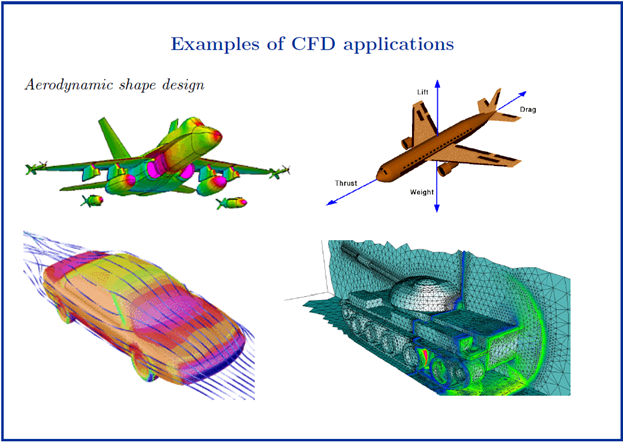
\includegraphics[width=.8\textwidth]{img/01/2.png}
\end{figure}
\begin{figure}[H]
    \centering
    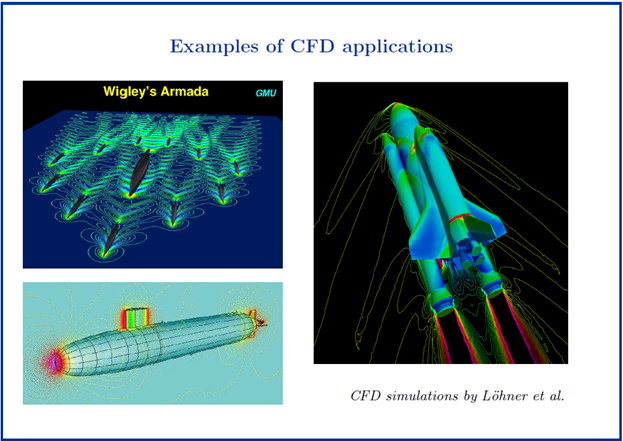
\includegraphics[width=.8\textwidth]{img/01/3.png}
\end{figure} 
\begin{figure}[H]
    \centering
    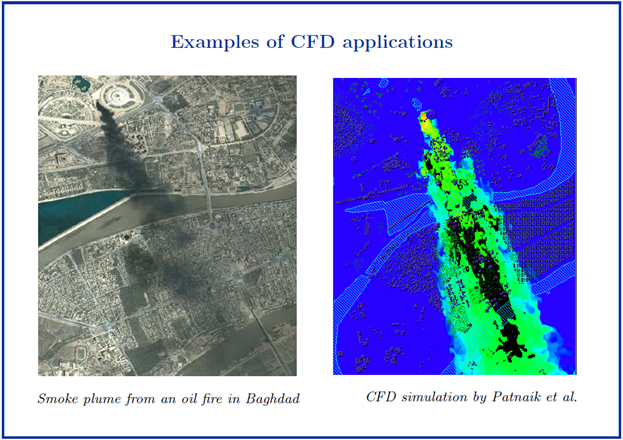
\includegraphics[width=.8\textwidth]{img/01/4.png}
    \caption{приклади використання обчислювальної гідродинаміки}
\end{figure} 

\subsection{Короткий історичний огляд}

\begin{itemize}
    \item[1910~р.] Л. Річардсон --- ітераційні методи розв'язку рівняння Лапласа, бігармонічного рівняння й інших рівнянь, уперше застосував чисельні методи до такої практичної задачі великого масштабу, як визначення напруг у кам'яній дамбі. 
    \item[1918~р.] Лібман вдосконалив метод за рахунок використання ``нових'' значень у вузлах, як тільки вони обчислені. 
    \item[1928~р.] Чисельний розрахунок гіперболічних рівнянь; метод характеристик; необхідна умова стійкості Куранта-Фрідріхса-Леві (КФЛ) (число Куранта повинне бути менше одиниці) справедливо для рівнянь гідродинаміки як у лагранжевих, так і в ейлерових змінних; з'явилася класична робота Куранта, Фрідріхса й Леві, що визначила напрямок практичного одержання скінченно-різницевих розв'язків у наступні роки.
    \item[1933~р.] Перший чисельний розв'язок рівнянь у частинних похідних для задач гідродинаміки в'язкої рідини було дано Томом в 1933 р.
    \item[1938~р.] Шортлі й Уеллер розробили вдосконалений варіант методу Лібмана, а також уперше точно визначили й досліджували швидкість збіжності.
    \item[1946--1948~рр.] Саусвелл і Фокс розробили схеми верхньої й нижньої релаксації.
    \item[1955~р.] Аллен і Саусвелл застосували метод релаксації Саусвелла для розрахунків вручну обтікання циліндра в'язкою нестислою рідиною. Були отримані чисельно стійкі розв'язки при числі Рейнольдса, рівному 1000, що перевищує фізичну межу стійкості. 
    \item[1950~р.] Франкел (і в 1954 р. незалежно від нього Янг) розробили метод, який згодом став називатися методом послідовної верхньої релаксації (назву запропонував Янг у 1954) або методом оптимальної верхньої релаксації. Франкел помітив також аналогію між ітеративним розв'язком еліптичних рівнянь і розв'язком кроками за часом параболічних рівнянь, що мало важливі наслідки.
    \item[1953~р.] Дюфорт і Франкел --- схема ``чехарда'' для параболічних рівнянь, яка, як і неявні схеми методу напрямків, що чергуються.
    \item[1955--1956~рр.] схеми методу змінних напрямків (Пісмен, Дуглас й Решфорд),
    \item[1957~р.] У першій монографії Ріхтмайєра, що була вагомим внесоком у розвиток одномірної нестаціонарної гідродинаміки, було наведено понад 10 чисельних схем. У багатомірному випадку першим неявним методом був метод Кранка-Ніклсона, опублікований в 1947 р., що й вимагав ітерацій на кожному часовому шарі. 
    \item фон Нейман (Лос-Аламос під час ІІ світової війни) --- критерій стійкості параболічних скінченно-різницевих рівнянь; метод дослідження лінеаризованої системи. 
\end{itemize}

\subsubsection{Гіперболічні рівняння}

\begin{itemize}
    \item[1960~р.] схема Лакса-Вендроффа.
    \item[1963~р.] схема Ріхтмайера.
    \item[1964~р.] методи PIC (метод часток в комірках), EIC (метод вибуху в гніздах), розроблені  Мадером, розмазування стрибків досягається за рахунок уведення кінцевого числа часток, що розраховуються. 
\end{itemize}

\subsubsection{Двокрокові методи}

\begin{itemize}
    \item Саульєв В.~К. запропонував двокроковий безумовно стійкий алгоритм, в якому в усіх просторових точках сітки на часовому кроці використовується явна схема, а на наступному кроці неявна. 
    \item Ідею двокрокового явно–неявного чисельного ``hорscotch'' методу, в якому, крім того, тип схем чергується і в просторових точках сітки, запропоновано Шелдоном для ітераційного роз-в'язування рівняння Пуассона. 
    \item Скала і Гордон  використали цю ідею для розв'язування задачі нестаціонарного обтікання кругового циліндра.
    \item Гурлі узагальнив її для нестаціонарного рівняння теплопровідності, довів стійкість. 
    \item В 1987 р. Грищенко О.~Ю розробив двокрокові-симетризовані алгоритми (ДС-алгоритми), поширивши ідею ``hорscotch'' методу на параболізовані лінійні і нелінійні задачі течії в'язкої рідини, переносу; для систем рівнянь першого порядку та систем газової динаміки, а також системи рівнянь Нав'є-Стокса. Ці алгоритми не потребують обернення матриці системи сіткових рівнянь.
\end{itemize}

\subsubsection{Грищенко Олександр Юхимович (1946--2016)}
\begin{itemize}
    \item з 1971 р. працював на кафедрі обчислювальної математики, проф., д.ф.-м.н.
    \item Опублікував понад 200 наукових та науково-методичних праць 
    \item Був членом спеціалізованої вченої ради із захисту докторських дисертацій КНУ імені Тараса Шевченка,  членом редакційної колегії ``Журналу обчислювальна та прикладна математика'' та головним редактором серії ``Прикладна математика'' цього ж журналу.
    \item Основні напрямки теоретичних досліджень пов'язані з 
    \begin{itemize}
        \item проблемами  побудови чисельних методів розв'язування крайових задач, 
        \item чисельного моделювання процесів динаміки та кінетики рідини, газу та плазми, 
        \item питаннями конструювання різницевих схем та чисельних алгоритмів із заданими властивостями, 
        \item розробкою чисельних методів, ефективних при розв'язуванні великих задач на багатопроцесорних комп'ютерних системах.
    \end{itemize}
    \item Результати цих досліджень впроваджувалися:
    \begin{itemize}
        \item при розрахунку та проектуванні фрагменту підземної частини насосної станції каналу Дніпро-Донбас
        \item моделюванні процесів очищення промислових стоків, 
        \item моделюванні робочих середовищ газодинамічних лазерів високої потужності та в інших прикладних проблемах.
    \end{itemize}
    \item Нагороди:
    \begin{itemize}
        \item У 1976 році за цикл робіт став лауреатом Премії імені М. Островського ЦК ЛКСМ України в галузі науки, техніки та виробництва.
        \item У 1978 році нагороджений дипломом третього ступеня МВССО України.
        \item У 2013 році премією Імені Тараса Шевченка Київського національного університету імені Тараса Шевченка.
        \item У 2015 році Почесною Грамотою Президії академії педагогічних наук \allowbreak України. Також нагороджений медаллю на честь 1500 річчя міста Києва.
    \end{itemize}
\end{itemize}
\newpage
\subsection{Апроксимація, збіжність і стійкість розв'язків}

\subsubsection{Апроксимація}

\begin{equation}
    \dfrac{\Delta f}{\Delta x} \xrightarrow[\Delta x \to 0]{} \dfrac{\diff f}{\diff x}.
\end{equation}

\begin{definition}
    \textit{Збіжна скінченно-різницева схема} математично визначається як схема, що дає скінченно-різницевий розв'язок, який збігається до розв'язку диференціального рівняння при прямуванні розміру комірки сітки ($\Delta x$) до нуля.
\end{definition}

\begin{remark}
    Під границею тут розуміється границя всього розв'язку диференціального рівняння, а не просто його окремих членів (похідних). 
\end{remark}

\begin{definition}
    Остання властивість називається \textit{апроксимацією} (Лакс й Ріхтмайер [1956]).
\end{definition}

\subsubsection{Стійкість}

о'Браян, Хаймен і Каплан [1950], а також Едді [1949] визначають стійкість виходячи з росту або загасання помилок округлення. Лакс й Ріхтмайер [1956] дають більш загальне визначення стійкості, установлюючи границю, до якої може зростати будь-який компонент початкових даних у процесі чисельного розрахунків.

\begin{theorem}[Лакса]
    Для системи лінійних рівнянь наявність стійкості є необхідною й достатньою умовою збіжності скінченно-різницевої схеми, що апроксимує систему диференціальних рівнянь.
\end{theorem}

\begin{theorem}[критерій стійкості фон Неймана]
    Вимагає, щоб найбільше власне значення матриці переходу ітераційної схеми було менше, чим одиниця мінус члени порядку помилки апроксимації.
\end{theorem}

Лакс й Ріхтмайер [1956] показали, що ця умова є достатньою для стійкості лінійної системи з постійними коефіцієнтами й що у випадку, коли матриця переходу задовольняє одному із трьох наборів властивостей, виконання цього критерію є достатнім також для збіжності.

\begin{remark}
    Дослідження лінійних рівнянь і рівнянь із постійними коефіцієнтами недостатньо для встановлення нестійкості. Визначення стійкості є неадекватним, оскільки для достатньо великого числа Рейнольдса при застосуванні стійких схем можуть виникати осциляції, що не мають нічого спільного із точним розв'язком.
\end{remark}

\subsection{Рівняння руху нестисливої рідини в декартовій системі координат}

\subsubsection{Рівняння руху для фізичних змінних}

\begin{definition}
    \textit{Рівняння Нав'є-Стокса}, що описують рух нестислої ньютонівської в'язкої рідини:
    \begin{equation}
        \frac{\partial \vec U}{\partial t} + \left(\vec U, \nabla \vec U\right) = - \frac{1}{\rho} \nabla P + \nu \Delta \vec U + \vec F,
    \end{equation}
    або, у 2-вимірному випадку:
    \begin{align}
        \label{eq:1.1}
        \frac{\partial \bar u}{\partial \bar t} + \bar u \frac{\partial \bar u}{\partial \bar x} + \bar v \frac{\partial \bar u}{\partial \bar y} &= - \frac{1}{\bar \rho} \frac{\partial \bar p}{\partial \bar x} + \bar \nu \left( \frac{\partial^2 \bar u}{\partial \bar x^2} + \frac{\partial^2 \bar u}{\partial \bar y^2} \right) + f_x, \\
        \label{eq:1.2}
        \frac{\partial \bar v}{\partial \bar t} + \bar u \frac{\partial \bar v}{\partial \bar x} + \bar v \frac{\partial \bar v}{\partial \bar y} &= - \frac{1}{\bar \rho} \frac{\partial \bar p}{\partial \bar y} + \bar \nu \left( \frac{\partial^2 \bar v}{\partial \bar x^2} + \frac{\partial^2 \bar v}{\partial \bar y^2} \right) + f_y, \\
        \label{eq:1.3}
        \frac{\partial \bar u}{\partial \bar x} + \frac{\partial \bar v}{\partial \bar y} &= 0.
    \end{align}
\end{definition}

\begin{remark}
    Риски над буквами означають, що відповідні величини є розмірними. Рівняння записані для фізичних змінних --- складових швидкості $u$, $v$ і тиску $p$; властивості рідини характеризуються щільністю $\rho$ і кінематичним коефіцієнтом в'язкості $\nu$.
\end{remark}
 
Ці рівняння засновані на наступних фізичних законах: рівняння \ref{eq:1.1} і \ref{eq:1.2} є проекціями векторного рівняння кількості руху $F = m a$ (другого закону Ньютона), причому сили в'язкості пов'язані зі швидкістю деформацій лінійним ньютонівським законом для дотичних напружень. Так, з другого закону Ньютона до елементарного об'єму рідини $\delta V$ масою $\delta m$ маємо:
\begin{equation}
    \delta m \frac{\diff \vec U}{\diff t} = \delta m \nu \Delta \vec U - \delta V \nabla P + \vec F \delta m.
\end{equation}
	 
У лівій частині формули --- добуток маси $\delta m$ елементарного об'єму рідини і її прискорення ($\vec U$ --- швидкість, $t$ --- час). У правій частині --- діючі на цей обсяг сили: сила в'язкого тертя ($\nu$ --- кінематична в'язкість), сила, що виникає через різницю тисків $P$, та інші сили $\vec F \delta m$.

\begin{remark}
    Рівняння \ref{eq:1.3} виражає закон збереження маси.
\end{remark}

\begin{definition}
    Наведені рівняння записані в \textit{ейлеровій} системі координат, тобто в нерухливій системі, щодо якої рухається рідина. 
\end{definition}

\subsubsection{Рівняння переносу вихору й рівняння для функції струму у випадку плоских течій}

З рівнянь \ref{eq:1.1} і \ref{eq:1.2} можна виключити тиск, продиференціювавши перше з них по $y$, а друге по $x$. Визначаючи \textit{вихор} як
\begin{equation}
    \label{eq:1.4}
    \bar \zeta = \frac{\partial \bar u}{\partial \bar y} - \frac{\partial \bar v}{\partial \bar x},
\end{equation}
одержуємо \textit{рівняння переносу вихору}, що має параболічний тип:
\begin{equation}
    \label{eq:1.5}
    \begin{aligned}
        \frac{\partial \bar \zeta}{\partial \bar t} &= -\bar u \frac{\partial \bar \zeta}{\partial \bar x} - \bar v \frac{\partial \bar \zeta}{\partial \bar y} + \bar \nu \left( \frac{\partial^2 \bar \zeta}{\partial \bar x^2} + \frac{\partial^2 \bar \zeta}{\partial \bar y^2} \right) = \\
        &= - \vec U \cdot (\nabla \bar \zeta) + \bar \nu \Delta \bar \zeta.
    \end{aligned}
\end{equation}

Використовуючи \textit{субстанціональну похідну} (Лагранжа)
\begin{equation}
    \dfrac{D \phi}{D t} = \dfrac{\partial \phi}{\partial t} + (\vec U \cdot \nabla) \phi,
\end{equation}
це рівняння можна представити так:
\begin{align}
    \label{eq:1.6}
    \frac{D \bar \zeta}{D \bar t} &= \vec U \Delta \bar \zeta \\
    \label{eq:1.7}
    \frac{\partial \bar \phi}{\partial \bar y} &= \bar u, \quad \frac{\partial \bar \phi}{\partial \bar x} = - \bar v,
\end{align}
рівняння \ref{eq:1.4} можна записати як рівняння Пуассона, що має еліптичний тип:
\begin{equation}
    \label{eq:1.8}
    \Delta \bar \phi = \bar \zeta.
\end{equation}

\subsubsection{Консервативна форма рівнянь}

Рівняння нерозривності \ref{eq:1.3}
\begin{equation}
    \frac{\partial \bar u}{\partial \bar x} + \frac{\partial \bar v}{\partial \bar y} = 0
\end{equation}
можна записати через вектор повної швидкості $\vec V$ в наступному виді:
\begin{equation}
    \label{eq:1.9}
    \nabla \cdot \vec V = 0.
\end{equation}

Використовуючи відому тотожність векторної алгебри
\begin{equation}
    \nabla  \cdot (\vec V \bar \zeta) = \vec V \cdot (\nabla \bar \zeta) + \bar \zeta (\nabla \cdot \vec V) = \vec V \cdot (\nabla \bar \zeta)
\end{equation}
одержуємо з \ref{eq:1.5} консервативну форму рівняння переносу вихору або \textit{дивергентну форму}
\begin{equation}
    \label{eq:1.10}
    \begin{aligned}
        \frac{\partial \bar \zeta}{\partial \bar t} &= - \nabla \cdot (\vec V \bar \zeta) + \bar \nu \Delta \bar \zeta = \\
        &= - \frac{\partial (\bar u \bar \zeta)}{\partial \bar x)} - \frac{\partial (\bar v \bar \zeta)}{\partial \bar y)} + \bar \nu \left( \frac{\partial^2 \bar \zeta}{\partial \bar x^2} + \frac{\partial^2 \bar \zeta}{\partial \bar y^2} \right).
    \end{aligned}
\end{equation}

\subsubsection{Рівняння в безрозмірних змінних}

Нехай $\bar L$ --- характерна довжина, а $\bar U_0$ --- характерна швидкість задачі.

\begin{example}
    Якщо $\bar L$ --- довжина хорди профілю крила й $\bar U_0$ --- швидкість потоку, що набігає, то $\bar L / \bar U_0$ --- час, за який частка потоку, що набігає, проходить увесь профіль. 
\end{example}

Уведемо наступні безрозмірні величини:
\begin{equation}
    \label{eq:1.11}
    u = \frac{\bar u}{\bar U_0}, \quad v = \frac{\bar v}{\bar U_0}, \quad x = \frac{\bar x}{\bar L}, \quad y = \frac{\bar y}{\bar L}, \quad  \zeta = \frac{\bar \zeta}{\bar U_0 / \bar L}, \quad t = \frac{\bar t}{\bar L / \bar U_0}.
\end{equation}

Тоді рівняння \ref{eq:1.10} і \ref{eq:1.8} приймуть вид
\begin{align}
    \label{eq:1.12}
    \frac{\partial \zeta}{\partial t} &= - \nabla \cdot (\vec V \zeta) + \frac{1}{\text{Re}} \Delta \zeta, \\
    \label{eq:1.13}
    \Delta \phi &= \zeta,
\end{align}
де $\text{Re}$ --- безрозмірний параметр, \textit{число Рейнольдса},
\begin{equation}
    \label{eq:1.14}
    \text{Re} = \bar U_0 \bar L / \bar \nu.
\end{equation}

Таким чином, для будь-якого заданого набору граничних умов течія характеризується одним безрозмірним параметром --- числом Рейнольдса. \medskip

Для течій з більшими числами Рейнольдса ($\text{Re} \gg 1$) конвективний член у рівнянні (\ref{eq:1.12}) превалює над членом в'язкої дифузії, і в цьому випадку величина $\bar L/\bar U_0$ буде являти собою інтервал часу, що фактично характеризує течію. Тоді, наприклад, умова для безрозмірного часу $t = \bar t / (\bar L / \bar U_0)$ буде підходящим критерієм для досягнення стаціонарного стану плину. Однак течія з малими числами Рейнольдса ($\text{Re} \ll 1$) краще характеризуються безрозмірним ``дифузійним'' часом. Визначаючи такий безрозмірний час як
\begin{equation}
    t' = \bar t \bar \nu / \bar L^2,
\end{equation}
а інші безрозмірні величини так само, як в \ref{eq:1.11}, одержуємо для функції струму те ж саме рівняння Пуассона \ref{eq:1.13}, але рівняння переносу вихору при цьому набуває вигляду
\begin{equation}
    \label{eq:1.16}
    \frac{\partial \zeta}{\partial t'} = - \text{Re} \nabla \cdot (\vec V \zeta) + \Delta \zeta.
\end{equation}

Величина $\bar \nu / \bar L^2$ має розмірність часу. Для того щоб оцінити її фізичну значимість як масштабу часу в завданнях з переважною дифузією, досить помітити, що в межі при $\text{Re} \to 0$ рівняння \ref{eq:1.12} стає сингулярним, тоді як рівняння \ref{eq:1.16} поводиться при цьому добре, а конвективний член зникає. Аналогічно, рівняння \ref{eq:1.12} не має особливості при $\text{Re} \to \infty$, але при цьому зникає дифузійний член $\ref{eq:1.16}$. 

\subsubsection{Одновимірні модельні рівняння переносу}

Рівняння переносу вихору як у неконсервативній, так і в консервативній формі \ref{eq:1.12} є параболічним за часом, містять дві незалежні просторові змінні й пов'язані з еліптичним рівнянням Пуассона для функції гока \ref{eq:1.13} через нелінійні конвективні члени.

\begin{enumerate}
    \item Лінеаризоване одновимірне рівняння з конвективним і дифузійним членами (Аллен [1968], У. Кроулі [1968]), записане або в консервативній формі
    \begin{equation}
        \label{eq:1.17}
        \frac{\partial \zeta}{\partial t} = - \frac{\partial (u \zeta)}{\partial x} + \alpha \frac{\partial^2 \zeta}{\partial x^2},
    \end{equation}
    або в неконсервативній формі
    \begin{equation}
        \label{eq:1.18}
        \frac{\partial \zeta}{\partial t} = - u \frac{\partial \zeta}{\partial x} + \alpha \frac{\partial^2 \zeta}{\partial x^2}.
    \end{equation}
    
    У цих рівняннях $\zeta$ моделює вихор або яку-небудь іншу конвективну й дифузійну величину, $\alpha$ --- узагальнений коефіцієнт дифузії, відповідний до величини $1/\text{Re}$ у рівнянні переносу вихору, $u$ --- лінеаризована швидкість конвекції, що не залежить від $x$, хоча рівняння \ref{eq:1.17} може бути використане й для вивчення ефектів стійкості у випадку, коли $u = u(x)$.

    \item Рівняння Бюргерса (Бюргерс [1948], Хопф [1950], Родін [1970]):
    \begin{equation}
        \label{eq:1.19}
        \frac{\partial u}{\partial t} = - u \frac{\partial u}{\partial x} + \alpha \frac{\partial^2 u}{\partial x^2},
    \end{equation}
    де $u$ розглядається як узагальнена швидкість. Це рівняння зберігає нелінійність рівняння переносу вихору й рівнянь Нав'є-Стокса. Завдяки своїй нелінійності воно може служити модельним рівнянням для вивчення як турбулентності, так і ударних хвиль. \medskip 

    Еквівалентна консервативна форма цього рівняння така:
    \begin{equation}
        \label{eq:1.20}
        \frac{\partial u}{\partial t} = - \frac{\partial}{\partial x} \frac{u^2}{2} + \alpha \frac{\partial^2 u}{\partial x^2},
    \end{equation}
    
    Оскільки відомі деякі аналітичні розв'язки рівняння Бюргерса, воно може служити для демонстрації переваг консервативної форми скінченно-різницевих рівнянь,
\end{enumerate}

\subsection{Завдання для самостійної роботи}

\shortHomeworkDescription{Встановити дивергентність системи рівнянь Нав'є-Стокса, записаних у змінних функція току-вихор. Побудувати систему обезрозмірювання для рівняння теплопровідності. Вказати умови, при яких дифузійне розповсюдження тепла переважає конвективне.}

